\section{Introduction}

A skeleton is a lower dimensional entity which represents shape of it's parent object. It being simpler than the parent object, operations like pattern recognition, approximation, similarity estimation, collision detection, animation, matching and deformation can be performed efficiently on it than on the parent object. 

Skeletons can be computed via various mathematical formulations such as Medial Axis Transform (MAT),  Chordal Axis Transform (CAT), Thinning etc. Table \ref{Medials} briefly summarizes these methods of Midcurves creation and their strengths-weaknesses.

\begin{table}
\caption{Current Medial Computation Methods}
\begin{tabular}[htbp]{@{} p{0.14\linewidth}  p{0.22\linewidth}  p{0.22\linewidth}  p{0.23\linewidth} @{}} \toprule
{\bf Method } & {\bf Medial }  & {\bf Description} & {\bf Comments}\\
\midrule
%------------------------------------------------------------------------------------------------------------------------------------
\raisebox{-.9\height}{MAT \cite{Ramanathan2004}} &
\raisebox{-.9\height}{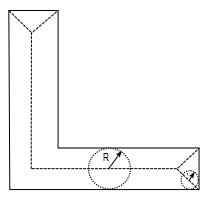
\includegraphics[scale=0.3]{..//Common/images/MAT.png} }&
Locii of centers of maximal disk traversing within boundary &
Computable for any shape. But has unwanted branches. Sensitive to boundary perturbations. \\


%------------------------------------------------------------------------------------------------------------------------------------
\raisebox{-.9\height}{CAT \cite{Quadros2008}}&
\raisebox{-.9\height}{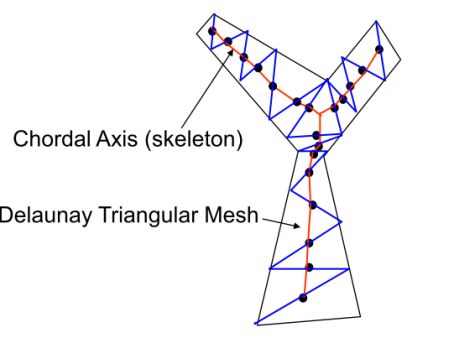
\includegraphics[scale=0.45]{..//Common/images/CAT.png}}&
Creates triangulation first then joins midpoints of sides &
Gaps at end. Expensive triangulation. \\


%------------------------------------------------------------------------------------------------------------------------------------
{Straight Skeleton \cite{Henrik2004}} &
\raisebox{-.9\height}{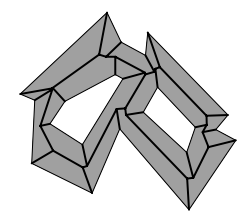
\includegraphics[scale=0.3]{..//Common/images/Straight.png}} &
Goes on thinning from boundary. &
Bisectors mot equidistant. Has unnecessary branches.\\

\bottomrule
\end{tabular}
\label{Medials}
\end{table}


In this paper we focus on 2D planar sketch profiles.  Even in 2D profiles, shapes vary enormously. At the first level of simplification, we would deal with 2D polygons only(with an assumption that curved shapes can be converted to polygonal shape by faceting). Divide-and-Conquer is one of the widely used strategy for dealing with complex models. Shape decomposition partitions given shape into sub-shapes and then skeletonization can be performed on simpler sub-polygons. 

A polygon can be decomposed into convex regions by dividing at all reflex(concave) vertices. Generally criterion for decomposition is to produce a minimum number of convex components or to minimize the total length of the boundary of these components. Within the minimum component criterion methods further classification could be based on whether or not Steiner points (brand new, non polygonal vertices) are allowed. 

